\documentclass[tikz,border=4pt]{standalone}
% Shared setup for the foundation-model diagrams, in the AFRICAST palette
\usepackage{fontspec}
\usepackage[sfdefault]{FiraSans}
\usepackage{amsmath}
\usepackage{unicode-math}
\setmathfont{Fira Math}
\usetikzlibrary{arrows.meta}
\definecolor{ink}{HTML}{1F2A36}
\definecolor{MonashBlue}{HTML}{3B75AC}
\definecolor{Orange}{HTML}{B5570F}
\color{ink}
\tikzset{every picture/.style={draw=ink,>=stealth}}
\hyphenpenalty=10000
\exhyphenpenalty=10000

\begin{document}
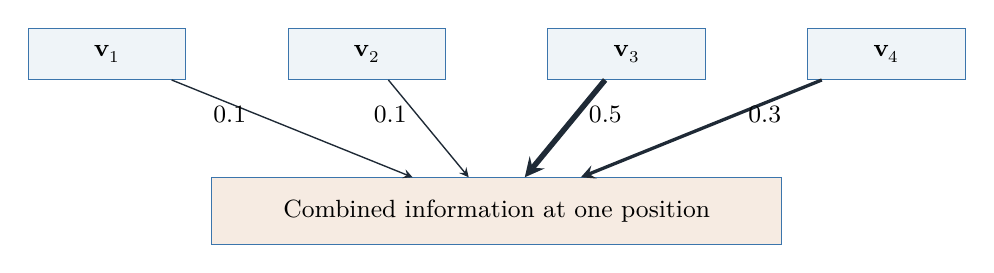
\begin{tikzpicture}[>=stealth,every node/.style={font=\fontsize{9}{10}\selectfont,align=center},
box/.style={draw=MonashBlue,fill=MonashBlue!8,minimum width=2cm,minimum height=.65cm}]
\node[box] (a) at (0,0) {$\mathbf{v}_1$};
\node[box] (b) at (3.3,0) {$\mathbf{v}_2$};
\node[box] (c) at (6.6,0) {$\mathbf{v}_3$};
\node[box] (d) at (9.9,0) {$\mathbf{v}_4$};
\node[draw=MonashBlue,fill=Orange!12,text width=7cm,minimum height=.85cm] (out) at (4.95,-2) {Combined information at one position};
\draw[->,line width=.5pt] (a)--node[pos=.35,left]{0.1}(out);
\draw[->,line width=.5pt] (b)--node[pos=.35,left]{0.1}(out);
\draw[->,line width=2pt] (c)--node[pos=.35,right]{0.5}(out);
\draw[->,line width=1.2pt] (d)--node[pos=.35,right]{0.3}(out);
\end{tikzpicture}
\end{document}
